\documentclass{wccm2014}

\usepackage{graphicx}
\usepackage{amsmath}
\usepackage{amsfonts}
\usepackage{amssymb}
\usepackage{subfig}
%%%%%%%%%%%%%%%%%%%%%%%%%%%%%%%%  MATH MACROS %%%%%%%%%%%%%%%%%%%%%%%%%%%%%%%%
\newcommand{\tr}{{\,\rm tr}\,}
\newcommand{\sen}{{\,\rm sen}\,}
\newcommand{\senh}{{\,\rm senh}\,}
\newcommand{\diverg}{{\,\rm div}\,}
\newcommand{\grad}{\,\mathbf{grad}\,}
\newcommand{\rot}{\,\mathbf{rot}\,}
\newcommand{\uvet}{\mathbf{u}}
\newcommand{\vvet}{\mathbf{v}}
\newcommand{\cvet}{\mathbf{c}}
\newcommand{\wvet}{\mathbf{w}}
\newcommand{\xvet}{\mathbf{x}}
\newcommand{\gvet}{\mathbf{g}}
\newcommand{\fvet}{\mathbf{f}}
\newcommand{\nvet}{\mathbf{n}}
\newcommand{\tvet}{\mathbf{t}}
\newcommand{\Imat}{\mathbf{I}}
\newcommand{\Eo}{\mathrm{Eo}}
\newcommand{\N}{\mathrm{N}}
\newcommand{\Mo}{\mathrm{Mo}}
\newcommand{\ca}{\cellcolor[gray]{0.5}}
\newcommand{\cb}{\cellcolor[gray]{0.0}}
%%%%%%%%%%%%%%%%%%%%%%%%%%%%%%%%%  -- END -- %%%%%%%%%%%%%%%%%%%%%%%%%%%%%%%%%


\title{TWO-PHASE FLOWS IN SINUSOIDALLY CONSTRICTED CHANNEL USING MOVING
MESH/BOUNDARY TECHNIQUE}

\author{GUSTAVO ANJOS$^{*}$, GUSTAVO OLIVEIRA$^{*}$, JOS\'E
PONTES$^{\dag}$, JOHN R. THOME$^{\dag}$ AND NORBERTO MANGIAVACCHI$^{*}$}

\heading{Gustavo Anjos, Gustavo Oliveira, Jose Pontes, John R. Thome,
Norberto Mangiavacchi}

\address{$^{*}$Mechanical Engineering Department/GESAR Group, State
University of Rio de Janeiro\\ R. Fonseca Teles 121, 20550-013, Rio de
Janeiro, RJ, Brazil\\ 
e-mail: gustavo.anjos@uerj.br, web page: http://gustavo.rabello.org
\and
$^{\dag}$Escola Polit\'ecnica/COPPE -- Universidade Federal do Rio de
Janeiro\\ P.O. Box 68505, Rio de Janeiro, RJ, 21941-972 Brasil\\
e-mail: jopontes@metalmat.ufrj.br
\and
$^{\dag}$EPFL STI IGM LTCM, ME B1 345, Station 9, CH-1015, Lausanne,
Switzerland\\
e-mail: john.thome@epfl.ch}

% NEED TO INCLUDE KEYWORDS!
\keywords{Finite Element Method, Arbitrary Lagrangian-Eulerian,sharp
interface, complex geometry, sinusoidal}

\abstract{ Bubbles and drops dynamics through capillaries of variable
cross-section still remains of considerable importantce in two-phase
flows through porous media. Experimental studies are found in the
literature where the motion of immiscible bubbles in different fluids is
investigated. Recovery of oil by chemical flooding, biological processes
and crude oil transportation in through pipelines are examples of
industry-related applications. We seek to study numerically the effects
of the surface tension, bubble dynamics and channel geometry for
two-phase flows in sinusoidally constricted channels using a moving
boundary domain scheme, which dramatically shortens the domain length.
Such a scheme moves the computational boundary nodes periodically
according to the flow field or bubble centroid's velocity. The set of
equations is written in a generalized form namely the Arbitrary
Lagrangian-Eulerian (ALE) description, which combines the best aspects
of both Lagrangian and Eulerian framework. The two-phase inteface
position moves according to the flow field and it is explicity described
by a set of interconnected nodes, segments and elements which ensures a
sharp representation of the front, not requiring the use of any
additional equation of motion \cite{anjos2012,anjos2014}. Unlike
the traditional numerical approach where the domain's boundary is fixed
in space and time, the boundary nodes are in constant motion, thus
simulating the relative velocity between the bubble and the wall. Such a
technique allows one to decrease considerable the domain length and,
therefore, decrease the computational processing time. The new
methodology proposed to simulate two-phase flows in sinusoidally
constricted channels is compared to experimental results found in the
literature \cite{olbricht1983,hemmat1996} showing good accuracy
to describe interfacial forces and bubble dynamics in different complex
geometries with moving boundaries.}

\begin{document}
%\maketitle

\section{INTRODUCTION}
\label{sec:intro}

Capillaries with variable cross-sections are used in enginnering
applications to incite unsteady behaviours in the kinematics of flows,
as opposed to the uniformity borne out in constant cross-sections
domains. Two-phase flow modelling in diverse geometries, were focused on 
studies upon enhanced oil recovery (EOR) techniques by chemical 
flooding \cite{olbricht1996,cobos2009}, pore-scale prototyping, 
evaluation of mobility control of immiscible fluids in porous media of 
subsurface \cite{hemmat1996}, and alteration of blood flow caused by 
vascular occlusions \cite{forrester1970}, for instance. In such problems
and like ones, converging/diverging tubes, sinusoidally constricted capillaries, as well as 
domains formed by a periodic pace of throats are extensively taken into account 
for their mathematical modelling.

A significant experimental insight about the influence of a tube with
wavy-wall geometry upon the dynamics of a droplet motion was given by
\cite{olbricht1983}, whereby they concluded that it depends strongly on
the capillary number. Moreover, they found that the pressure drop of the
droplet is always associated to the constrictions of the tube, which,
for a real porous media, would be tied to the retention of bubbles at
determined sites and their consequent low mobility. Comparatively, the
pore plugging phenomenon, by which trapped droplets hinder the overall
permeability of the medium, was faced by \cite{graham2000} through
acoustic stimulation. Their results showed efficiency as to
remobilization processes and good capabilities for application in
several industrial operations, such as filtration issues, flow in packed
beds, and the manufacture of fibrous composites. Drop breakup in
constricted capillaries, or \emph{snap-off} effects, is an appreciated
issue \cite{tsai1994}. Apart from these, recent research was also
carried out in diverging/converging geometries to examine heat transfer
characteristics of suspensions and polymers \cite{narayanam2014}, which
awakens a wide range of interest upon these flows.

With attention to computational works propping up the investigation of
the motion of disperse elements through narrow passages and bottlenecks,
techniques relied on finite volume/front-tracking were introduced in the
modelling of buoyancy-driven viscous drop through constricted
capillaries, where the interfaces were represented by using connected
Lagrangian marker points which move with the local flow velocity
\cite{muradoglu2006,olgac2006}. More
recently, implementations gathering finite element/level-set methods
also were performed in order to elucidate the dynamics of drops inside
constricted microcapillaries headed to industrial purposes as regards
oil-water emulsions, mobility control, and pressure drop, for instance
\cite{roca2013}. 

In this work, we seek to study numerically the effects of surface
tension, bubble dynamics, and geometry on two-phase flows in
sinusoidally constricted channels by using a moving boundary domain
scheme, which shortens the domain length dramatically. Such scheme moves
the computational boundary nodes periodically according to the flow
field or the bubble centroid's velocity. The set of equations is written
in a generalized form, namely the Arbitrary Lagrangian-Eulerian (ALE)
description, so combining the best aspects of both Lagrangian and
Eulerian descriptions. To model the interface between the phases, we
allow that the points over it move according to the flow field. In turn,
the interface is explicitly described by a set of interconnected nodes,
segments, and elements so ensuring a sharp representation of the front
and supplanting the use of any additional equation to govern the movement
of interface points \cite{anjos2012,anjos2014}. Unlike the
traditional numerical approach where the domain's boundary is fixed in
space and time, the boundary nodes are kept in constant motion, thus
simulating the relative velocity between the bubble and the wall.
Moreover, the results are obtained over a reduced computational domain,
which, therefore, implies a smaller computational processing time.

The paper is organized as follows: Sec.~(\ref{sec:governing}) exposes
briefly the set of equations governing the physical problem;
Sec.~(\ref{sec:ale}) gives an overview of the ALE formulation
implemented; Sec.~(\ref{sec:results}) introduces the results obtained,
and, in last, conclusions are drawn in Sec.~(\ref{sec:conclusions}). 

%--------------------------------------------------
% A displayed equation is numbered, using Arabic numbers in
% parentheses. It should be centered, leaving a 6pt space above and
% below to separate it from the surrounding text.
% The following example is a single line equation:
% \vskip-.6cm
% \begin{eqnarray}
% Ax = b
% \end{eqnarray}
% The next example is a multi-line equation:
% \vskip-.6cm
% \begin{eqnarray}
% Ax = b \\
% Ax = b \nonumber
% \end{eqnarray}
%-------------------------------------------------- 
\section{MATHEMATICAL FORMULATION}
\label{sec:governing}

For the mathematical description of the problem, it suffices to follow up the illustration provided by Fig. \ref{fig:domain}, which represents the central cut plane perpendicular to the sinusoidal tube. Consider $ \Omega^1 $ the region of the domain occupied by the vapour phase and $ \Omega^2 $ the complementary, associated to the liquid phase. The tube constrictions bound the fluid portion obeying a waveform function given by $ a(x) $, whose parameters $ a_0 $, $ a $, $ \phi $, $ n $, and $ \alpha $ are, respectively, an initial wave amplitude (conveniently chosen to be zero herein), the wave amplitude, the phase angle, the number of periods, and a stretching factor. The two latter parameters control the wavelength so allowing certain flexibility to mesh design and adjustment. $ P $ is the variable related to the longitudinal periodic length, while $ R $ is a mean radius for the tube. 
\begin{figure}
\centering
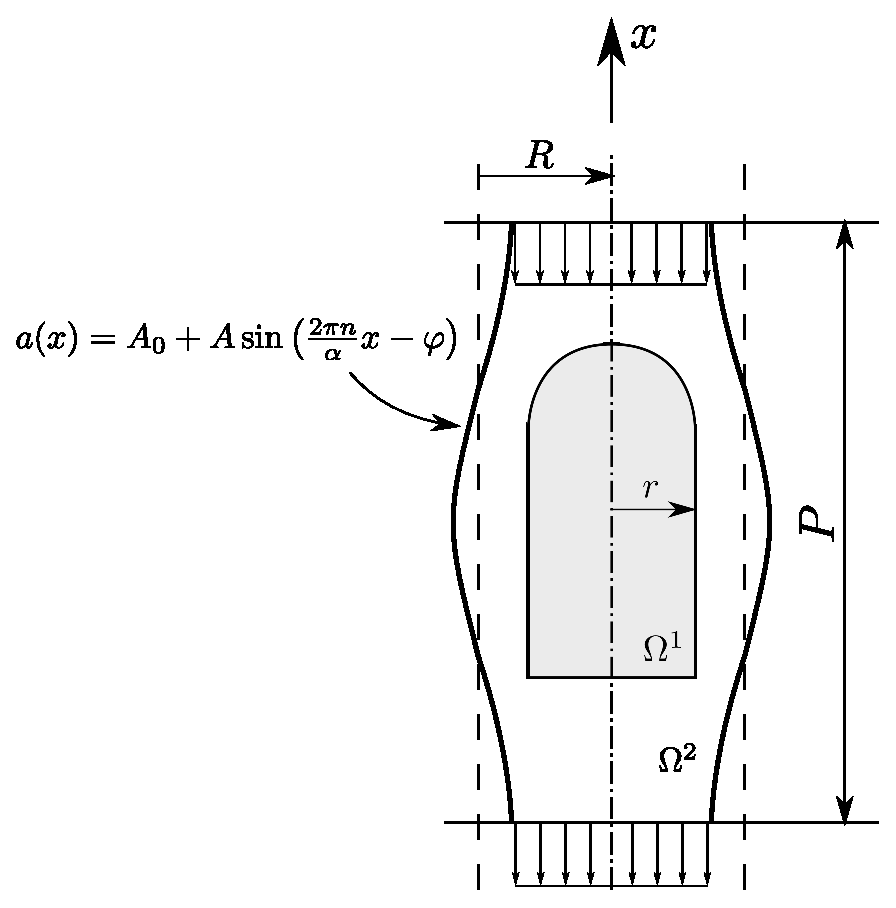
\includegraphics[scale=0.5]{figs/eps/profile-tube-bubble.eps}
\caption{\label{fig:domain}Schematic of the central cut plane for the sinusoidally constricted domain.}
\end{figure}
The vapour phase is made up by a Taylor bubble of radius $ r $, whose dynamics we are intended to analyse. In virtue of a moving-frame technique, the transit of the bubble through the bottlenecks is locally evaluated by observing the topological changes on the bubble's surface. At the top and bottom cross sections, the liquid velocity is essentially uniform, being that, an equivalent buoyancy-driven flow produced with the application of a pressure gradient contrary to the bubble's motion establishes an outflow condition downhill. \marginpar{GCPO: Gustavo, pls, check the parameters setting (n,$\phi$,...).}

The non-dimensional incompressible conservation equations for two-phase
flows is presented below through the generalized Arbitrary
Lagrangian-Eulerian (ALE) framework including the surface tension term
$\mathbf{f}$ and the gravity term $\mathbf{g}$: 

\begin{equation}
	\rho(\phi) [ \frac{\partial \uvet}{\partial t} 
	+ \cvet \cdot \nabla \uvet ]
	=
	- \nabla p 
	+ \frac{1}{\N^{1/2}} \nabla \cdot
	[\mu(\phi) ( \nabla \uvet + \nabla \uvet^T)]+
	\rho(\phi) \mathbf{g}+
	\frac{1}{\Eo} \mathbf{f}
	\label{eq:nd-momentum}
\end{equation}

\begin{equation}
	\nabla \cdot \uvet
	= 
	0.
\label{eq:nd-continuity} 
\end{equation}

On the left hand side of Eq.~\ref{eq:nd-momentum}, the convective velocity
$\cvet$ represents the relative velocity between the flow field and the
mesh, given by the following expression: $\cvet = \uvet - \hat{\uvet}$
where $\uvet$ stands for the computed flow field velocity and
$\hat{\uvet}$ for the mesh velocity. Pressure is represented by $p$ and
time by $t$. The fluid density $\rho(\phi)$ and viscosity $\mu(\phi)$
are defined as constant in each phase. The non-dimensional groups
\textit{Archimedes} and \textit{E\"otv\"os} are defined as follow:

\begin{equation}
 \N = \frac{\rho_0^2 D^3 g}{\mu_0^2},
 \Eo = \frac{\rho_0 g D^2}{\sigma_0},
 \Mo = \frac{(\rho_l-\rho_g)\mu_0^4 g}{\rho_{0}^2 \sigma_0^3} 
 \label{eq:nd-groups}
\end{equation}


%%% SUBSECTION EX.: \subsection{Example}
\section{NUMERICAL RESULTS}
\label{sec:results}

\subsection{Sessile drop}
\label{sessile}
The next simulation was performed to validate the surface tension
implementation and its coupling with pressure and gravity. A spherical
drop with radius $R=0.5$ was initialized two diameters above the bottom
of the domain and then released. Due to gravity, the drop, being 
heavier than the surrounding fluid, falls and hits the solid surface.
Before the contact between the solid surface and the interface, the drop
deforms to a quasi-steady state and approaches the wall with no
significant shape changes. The drop's profile remains axisymmetric and
its shape can be approximated by the classical Young-Laplace equation of 
capillarity which, in non-dimensional form, states that:

\begin{equation}
	\big( \frac{1}{R_1}+\frac{1}{R_2} \big)\frac{1}{Eo}
	=
	\Delta p_g
	=
	\Delta \rho g (z-z_0)
	\label{eq:young-laplace}
\end{equation}

\noindent where $R_1$ and $R_2$ are the two principal radii at the apex
of the drop, $\sigma$ is the interfacial tension and $\Delta p_g$ stands
for the hydrostatic pressure difference across the interface, where
$\Delta \rho = \rho_{in}-\rho_{out}$. Considering $\phi$ as the drop
tangent angle with respect to the wall, for an axisymmetric drop:

\begin{equation}
	\big( \frac{1}{R_1}+\frac{1}{R_2} \big)
	=
	\kappa 
	= 
	\frac{d\phi}{ds} + \frac{\sin \phi}{r} 
	\label{eq:yl2}
\end{equation}

\noindent where $s$ is the coordinate along the surface and $r$ is
the radial coordinate. Substituting Eq.~(\ref{eq:yl2}) into 
Eq.~(\ref{eq:young-laplace}), results in:

\begin{equation}
	\frac{d \phi}{ds} = 
	\hat{\Eo}(p-z) - \frac{\sin \phi}{r}
	\label{eq:sessile1}
\end{equation}

\begin{equation}
	\frac{dr}{ds} = \cos \phi
	\label{eq:sessile2}
\end{equation}

\begin{equation}
	\frac{dz}{ds} = \sin \phi
	\label{eq:sessile3}
\end{equation}

\noindent Here, $\hat{p}$ stands for the dimensional reference pressure,
$p=\hat{p}/\rho g L$ as the non-dimensional pressure and $\hat
{\Eo}=\Eo(\Delta \rho/\rho_{in})$ as the modified \textit{E\"otv\"os}
number. These equations are solved using a forth order Runge-Kutta method with
appropriate initial conditions: $s=0$, $\phi=0$, $r=0.258$ and $z=0$ and
then solved and integrated up to $\phi=\pi$. The solution of the
ordinary differential equations presented from \ref{eq:sessile1} to
\ref{eq:sessile3} are used to benchmark the numerical solution given by
the presented ALE-FEM two-phase flows code.

% and pressure due to the curvature
% $P_{\sigma}=2 \sigma / r$. 
% 
% For an axisymmetric drop, $R_1=R_2=r$ where
% $r$ is the radius of curvature at the apex. 

% simulation conditions
The simulation of the drop for three different mesh refinement levels
($h={0.12,0.06,0.03}$) was performed assuming the following
non-dimensional parameters: $R=0.5$, $\Eo=2$, $\rho_{in}=1.0$ and
$\mu_{in}=1.0$ for the drop and $\rho_{out}=0.1$ and $\mu_{out}=0.9$ for
the external fluid. The domain limits were set to be
$8D\text{x}8D\text{x}4D$, where the last dimension stands for the
direction of gravity, and discretized by approximately $26000$
tetrahedrons and $5100$ nodes. The interface mesh had approximately
$5400$ triangles in which $2056$ were part of the interface mesh. The
mesh parameters used were $\beta_1=0$, $\beta_2=1.0$, $\beta_3=1.0$,
$\gamma_1=0.1$ and $\gamma_2=0.0$, thus keeping the volumetric and
surface meshes as well as the distance of nodes to the surface elements
almost uniform while the drop is moving downward to the bottom of the
domain. The final solution of the sessile drop test case
can be seen in Fig.~(\ref{fig:sessileMesh}), where the background mesh
was intentionally sliced to show the background tetrahedron faces and
the triangular surface mesh of the axisymmetric drop with $h=0.06$.
Figure~(\ref{fig:sessileKappa}) shows the curvature distribution along
the drop's height. The solid line was fit using the data from
$z=[0.2,0.8]$ by the least squares method; therefore the slope of such a
line gives the value of $\hat{\Eo}=2$ for which it can be used to solve
the previous mentioned ODE. Additionally, comparing the distance from
the numerical data to the solid line, it is possible to compute the
error of curvature for the simulated drop. Thus, the curvature error
$\text{Error}_{\kappa}$ was found to be $0.2$, showing reasonable
agreement to the analytical solution. Furthermore, the numerical
solution of the drop's shape is compared to the semi-analytical solution
of the Young-Laplace's equation
(Eqs.~(\ref{eq:sessile1})--(\ref{eq:sessile3}))
and is shown in Fig.~(\ref{fig:sessileShape}). The results show that the
sessile drop is correctly predicted by the present implementation, due
to the accurate balance of the gravity, pressure and surface tension
forces.

\begin{figure}[ht!]
	\begin{center}
		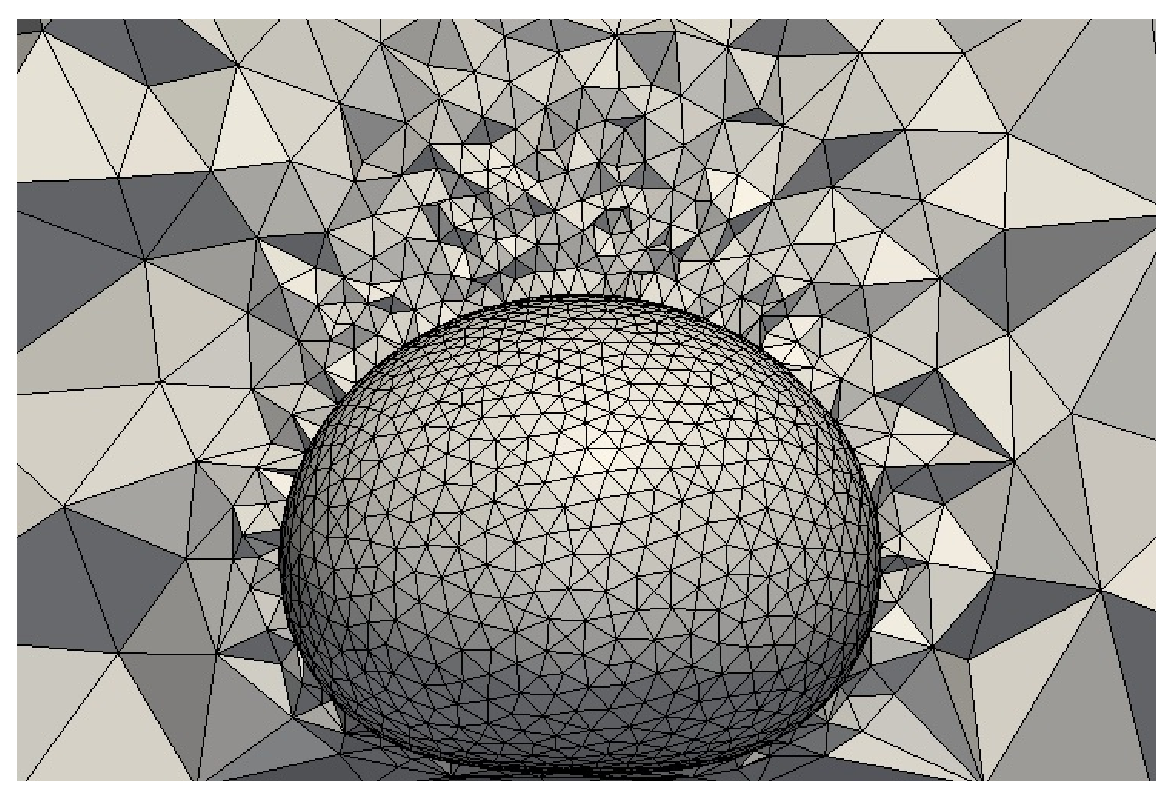
\includegraphics[angle=0, scale=0.5]{figs/eps/sessileMesh.eps}
	\end{center}
	\caption{Numerical solution of the sessile drop test
	case. The tetrahedron faces of a cut-plane background mesh and the
	triangular surface mesh ($h=0.06$) are shown to illustrate the last
	time step, whose shape is used to compare with the analytical
	solution given by Eqs.(\ref{eq:sessile1}--\ref{eq:sessile3}).}
	\label{fig:sessileMesh} 
\end{figure}

\begin{figure}[ht!]
	\begin{center}
		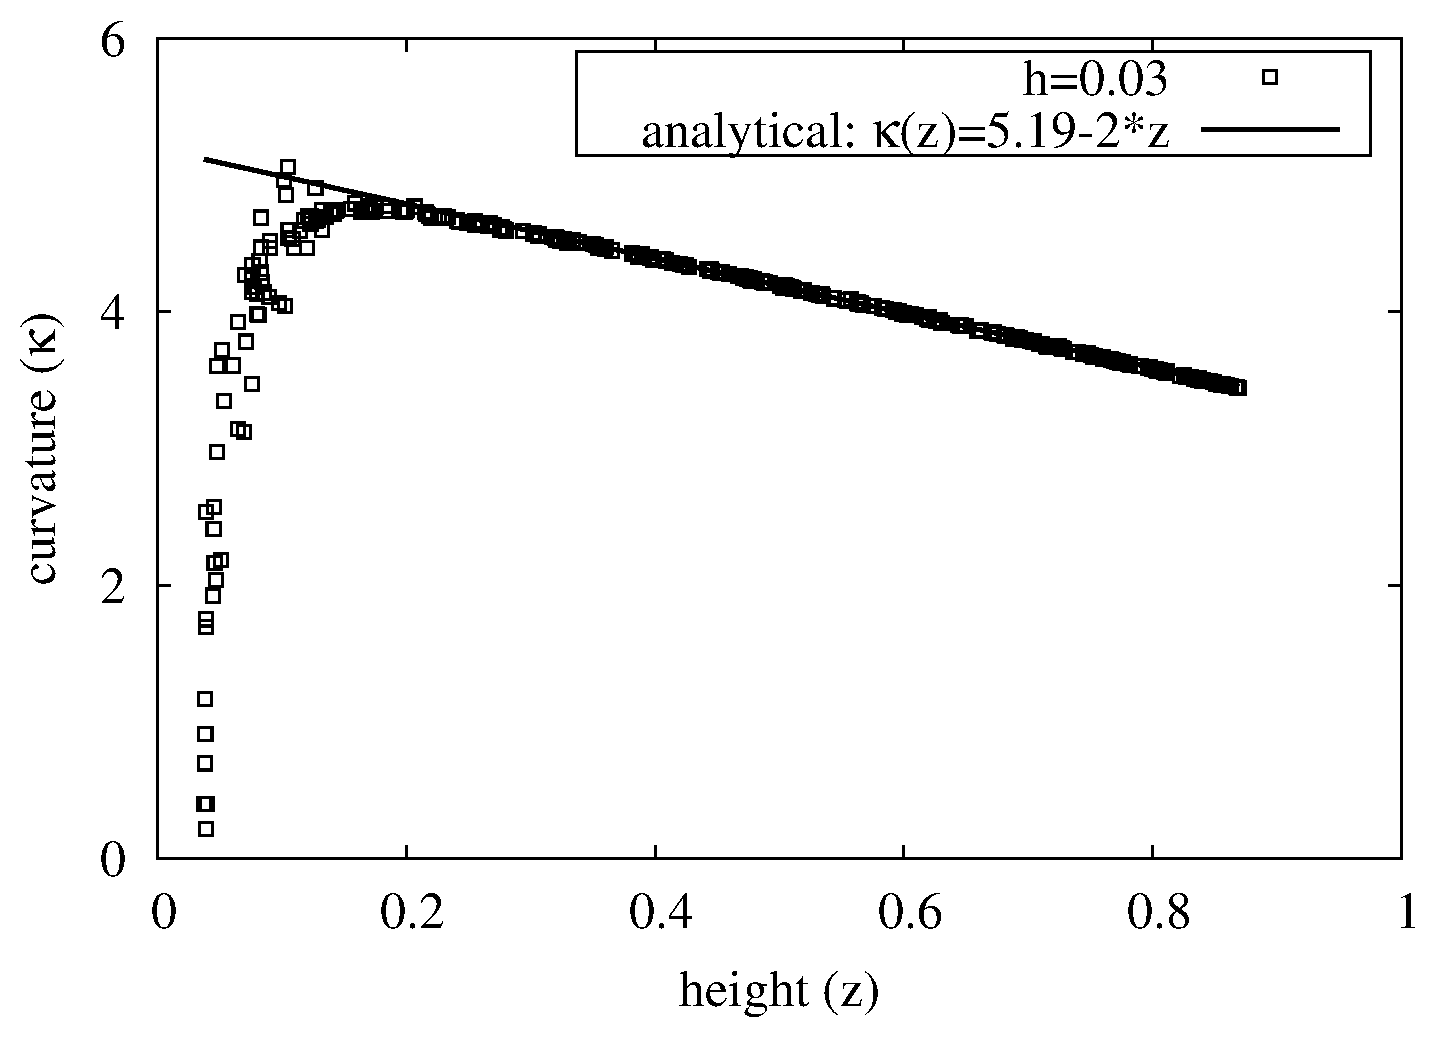
\includegraphics[angle=0, scale=0.5]{figs/eps/sessileKappa.eps}
	\end{center}
	\caption{Curvature distribution along the drop's height. The solid
	line was fit by the least square method and its slope gives the value 
	of $\hat{\Eo}=2$.}
	\label{fig:sessileKappa} 
\end{figure}

\begin{figure}[ht!]
	\begin{center}
		\subfloat[]{
		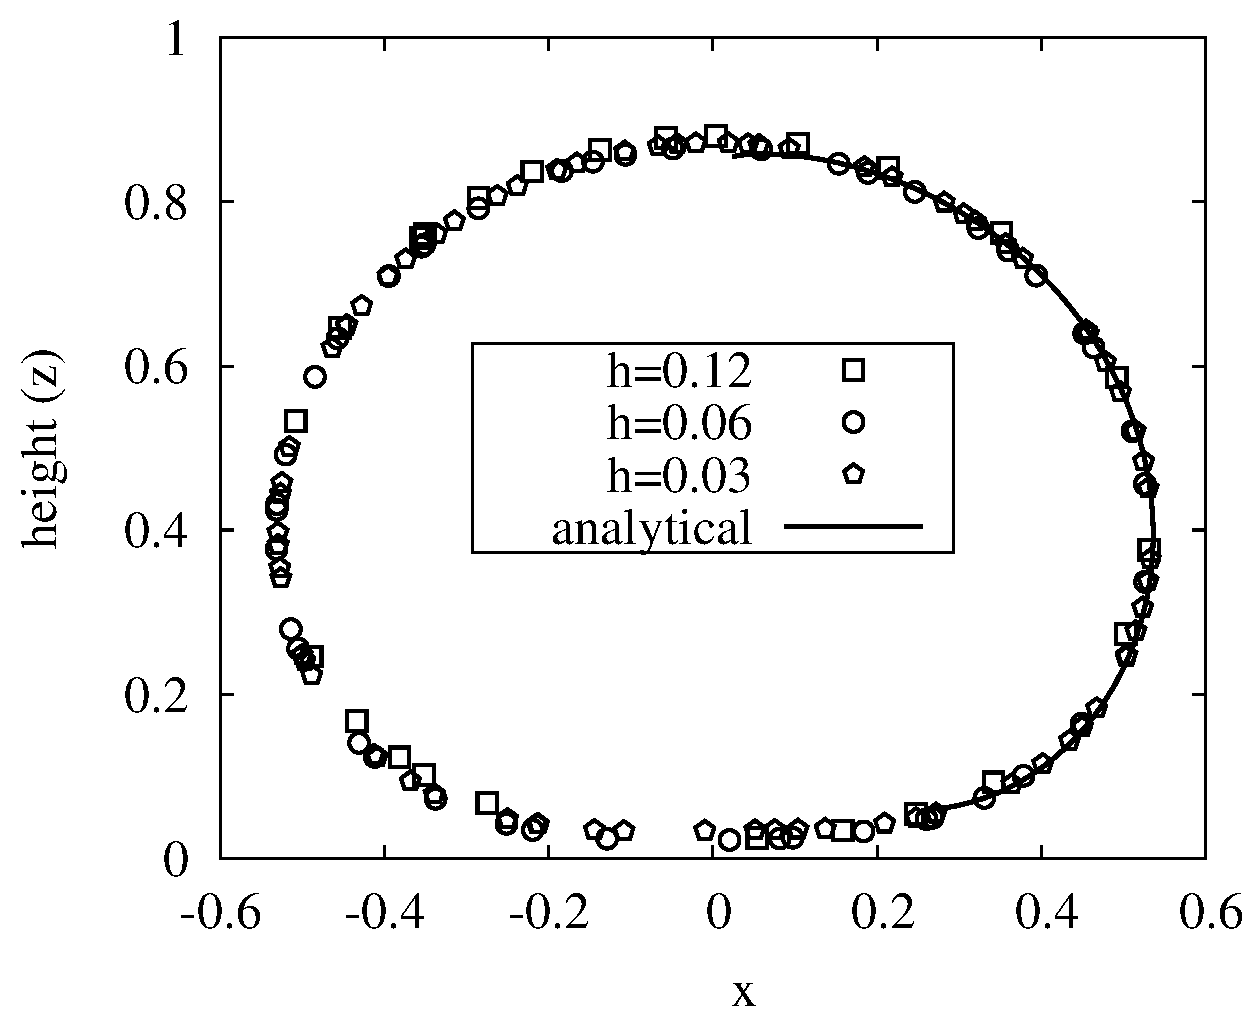
\includegraphics[angle=0, scale=0.43]{figs/eps/sessileShape.eps}}
		\subfloat[]{
		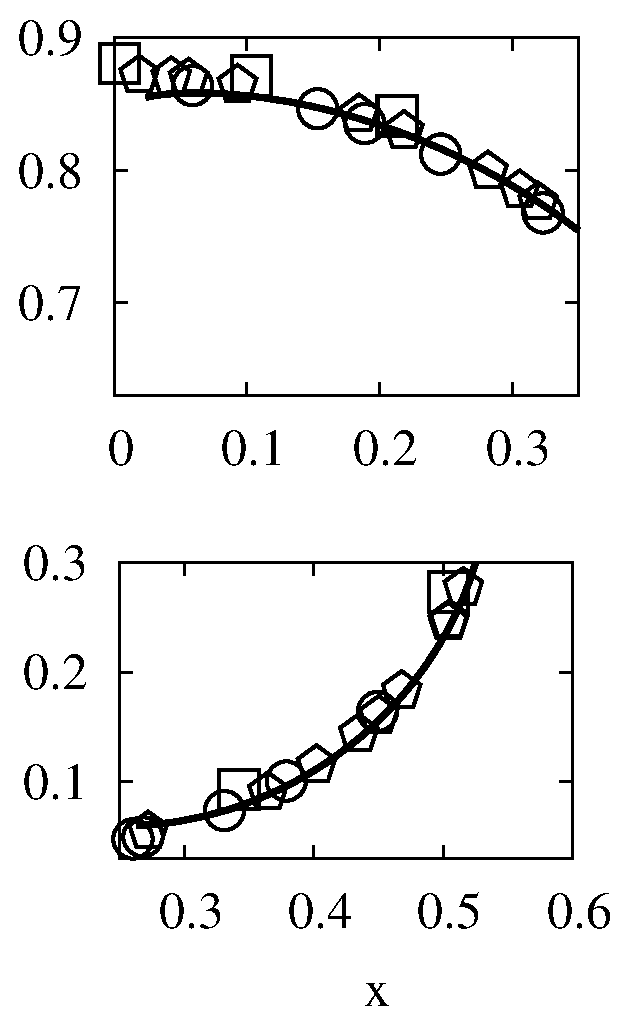
\includegraphics[angle=0, scale=0.43]{figs/eps/sessileShapeZoom.eps}}
	\end{center}
	\caption{(a) Comparison between the numerical solution for
	 different mesh refinement levels of an 3-dimensional axisymmetric
	 sessile drop and the analytical solution of its shape derived by
	 the Young-Laplace equation of capillarity. (b) Detailed view of the
	3-dimensional drop for $0.25<x<0.6$ (bottom part) and for $0<x<0.35$
  (upper part). }
	\label{fig:sessileShape} 
\end{figure}

\section{CONCLUSIONS}
\label{sec:conclusions}
This is the conclusions section
\section{ACKNOWLEDGEMENTS}
\label{sec:acknowledgements}
This research is funded by the brazilian research funding agency CAPES
in the scholarship program Science without Borders.

% BIBLIOGRAPHY EXAMPLE
\bibliographystyle{plain}
\bibliography{bibliography}

%--------------------------------------------------
% \begin{thebibliography}{99}
% BIBLIOGRAPHY EXAMPLE
% \bibitem{Zienkiewicz}  Zienkiewicz, O.C. and  Taylor, R.L. \textit{The finite element method}. McGraw Hill,
% Vol. I., (1989), Vol. II., (1991).
% \bibitem{Idelsohn} Idelsohn, S.R. and O\~{n}ate, E. Finite element and finite volumes. Two good friends.
% \textit{Int. J. Num. Meth. Engng.} (1994) \textbf{37}:3323--3341.
% \end{thebibliography}
%-------------------------------------------------- 


\end{document}


